\chapter{Tipi generici e collezioni}

Si vuole poter lavorare in modo "safe" con i tipi di dati senza dover costantemente controllare i tipi di dato.

\section{Tipi generici}

\dfn{Tipi generici}{
I tipi generici si usano per scrivere codice generico applicabile a più tipi di dati (riusabilità del codice). Il tipo E fa un match con qualunque tipo di dato non primitivo al momento della compilazione.

I generici sono stati introdotti per fare inferenza in fase di type checking statico.
}

\nt{Solitamente per i tipi generici si usa la lettera E, ma è solo una convenzione. Qualunque lettera va bene.}

\nt{Si potrebbe usare il tipo Object, ma ciò ha delle limitazioni: per esempio, in un array, possono essere inseriti elementi di tipi diversi. Ovviamente si può usare la reflection, ma ciò è scomodo e inefficiente.}

\ex{ArrayList}{
La classe ArrayList è generica, per cui può contenere oggetti di qualunque tipo. Tuttavia se non si specifica il tipo (ArrayList a = new ArrayList();) verrà considerato Object causando i problemi visti sopra.
}

\dfn{Tipi parametrici}{
Un tipo parametrico è una classe in cui è specificato il tipo generico da inferire.
}

\ex{ArrayList parametrico}{ArrayList$<$Double$>$ a = new ArrayList$<$Double$>$;}

\nt{Si possono creare classi generiche mettendo il parametro E nel nome della classe ($<$E$>$).}

\dfn{Tipo grezzo}{Il compilatore non ragiona in termini di tipi generici. Quindi il compilatore li trasforma in tipi grezzi (raw types), ossia unicamente il tipo della classe senza i parametri.}

\ex{ArrayList}{Quindi: 

ArrayList$<$String$>$ a = new ArrayList$<$String$>$

ArrayList$<$Double$>$ a = new ArrayList$<$Double$>$

hanno lo stesso tipo ArrayList.
}

\nt{Non si possono avere metodi statici con tipi generici all'interno delle classi che usano quei tipi.}

\section{Collezioni}

\dfn{Collezioni}{
Java fornisce un insieme di classi che realizzano strutture dati utili (le collezioni), come 
liste o insiemi.
}

\begin{figure}[h]
    \caption{Le collezioni}
    \begin{center}
        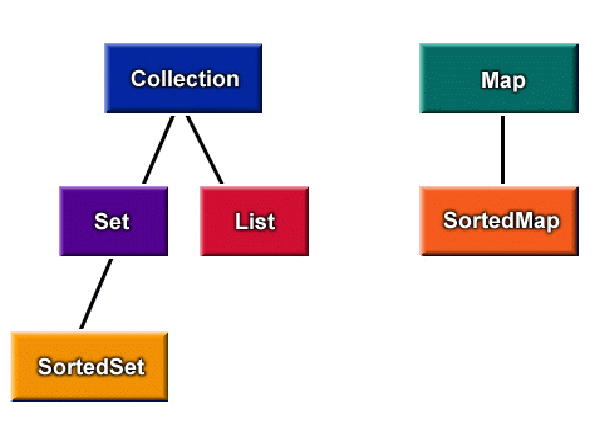
\includegraphics[scale=0.35]{images/Tipi generici e collezioni/Collezioni.png}
    \end{center}
\end{figure}

\nt{Queste sono tutte interfacce:
    \begin{itemize}
    \item \textbf{Collection}: un arbitrario gruppo di oggetti;
    \item \textbf{List}: un gruppo ordinato di oggetti;
    \item \textbf{Set}: un gruppo di oggetti senza duplicati;
    \item \textbf{Map}: una collezione di coppie chiave-valore.
\end{itemize}}

\dfn{Iteratori}{
Un iteratore è un oggetto che permette di scorrere una collezione, ottenendo gli elementi uno alla volta.
Il metodo iterator<> della classe Collection restituisce un iteratore per la collezione.
Si può "ciclare" su una collezione usando un iteratore con next() o con il for each.
}

\nt{Gli array mantengono sempre il loro tipo (a runtime), mentre le collezioni no.}

\dfn{Il tipo jolly (wildcard)}{
Per definire una collection di qualunque generico su usa la notazione collection$<$?$>$.
In una collezione di ? non si può aggiungere nulla, ma si può rimuovere.
}